\documentclass[a4paper, 10pt]{article}
\usepackage{graphicx}
\usepackage{listings}
\lstset{basicstyle=\ttfamily}
\usepackage{multirow} 
\usepackage{subcaption}
\usepackage{url} 
\usepackage{lipsum} 
\usepackage[]{mdframed}

[Incomplete] Note shuffling in progress, sources incoming... \\
\title{``Raspberry Pi Introduction'' Standard Notes}
\date{2021-2023}

\setlength{\parindent}{0pt}
\begin{document}
\maketitle

\pagebreak

\tableofcontents

 %=============================================================
 \pagebreak

\section{``READ ME FIRST''}
	\subsection*{``Warnings going forward''}
		\subsubsection*{Summary}
		There are instructions that must be known. Some terminology will be unknown, but will be explained when the time comes. 
	
		\subsubsection{Properly shutting off the RP}
            Do NOT unplug the raspberry pi to power off. This may corrupt the SD card, and require it be reflashed. 
            \textit{(Thankfully, the Ubuntu OS is much less prone to corruption than Raspbian)}.\\

            The RP can be shut off with the following command:
            \begin{lstlisting}[language=bash]
                sudo shutdown -h now
            \end{lstlisting}       
            Wait until the green and red LEDS (next to the power port) fully stop flashing before unplugging the RP.\\

            When the raspberry pi first boots, it may take 5 minutes before you notice a response. This is fine. \textbf{Do not unplug}.

		\subsubsection{Know thee voltages}
            - Power\\
            - GPIO pins\\
            - Everything\\

            \subsubsection{Don't edit just any file}
            If you don't know what you are doing, feel unsure, or the file specify "\textit{don't edit here please :)}", then DO NOT edit the files!\\

            Unless you really know what you are doing, this is for you:\\
            Don't touch .config files.\\
            Don't change configuration settings to force something to work. If a process or tutorial is overly convoluted, it may be a bad idea.\\
            Don't work on something at 2 AM.

            \subsubsection{Be patient with the boot}
            It can take the raspberry pi up to 5 minutes to finish it's first boot. It's fine, do not try to turn it off.

            While the raspberry pi is booting, be careful not to hit any keys, as it may stop the auto boot.

 %=============================================================
 

 \pagebreak


\section{``Common Linux Commands''}
		\subsubsection*{Note}
		This section is listed first since it's a prerequisite for           configuring and using the raspberry pi, however it's not             necessary to read this first.
            We'd recommend first skimming this section then treating it as a manual when needed.

            \subsubsection*{Summary}
            Linux commands will be heavily used to access and navigate through the raspberry pi, especially (but not limited to) when an OS is installed as a server rather than a desktop.
	
		\subsubsection{What is sudo?}

		\subsubsection{Navigating directories}
		A directory is ..
            - ls
            - cd

            \subsubsection{Creating, editing and executing code}
            - echo
            - nano
            - python3

            \subsubsection{SSH}
            - SSH
            - Adding -v, -vv, -vvv (etc) for debugging
            - X11 Forwarding

	\subsection{References/Resources}
 %=============================================================
\pagebreak


\section{``The Raspberry Pi''}
    \subsection*{Summary}
    This section covers ...
	
    \subsection{What is the raspberry pi?}

    The Arduino is a \textbf{micro-controller} with a simple \textbf{Integrated Circuit} (IC) chip. It can be fed Arduino code and loop through it infinitely until specified to stop. It has no OS utilities, but not to be underestimated, it has been used to build very simple web servers. \\
    
    One the other hand, the raspberry pi is a full-fledged computer in that most models contain the following:
    \begin{itemize}
      \item GPU: Graphics Processing Unit. 
      \item CPU: Central Processing Unit.
      \item Storage: Used for long-term data storage. This can include hard disk drivers, USB drives, and etc. Although data remains stored after a computer is turned off, it's slow to send/receive data.
      \item RAM: Random Access Memory is used for short-term data storage. It's much faster than Storage for sending/retrieving data, so computers with more RAM tend to run faster and allow more programs to run together.
      \item In/Outputs: There are multiple connectivity options:
        \begin{itemize}
          \item Power source: The RP 4 uses a USB-C power supply, and other models use a micro-USB power supply. Check the voltage requirements of the specific model before plugging. 
          \item SD card slot: The most important feature. Allows the user to burn an OS on the SD card, then mount it on the raspberry pi. It can also be used for storage.
          \item USB ports: These can be used for USB or keyboard/mice dongles.
          \item HDMI port: HDMI (High-Definition Multimedia Interface) can be used to transmit video & audio to a monitor for display.
          \item Specified ribbon cable connectors: The connectors are labeled for their specific function (Display/Camera), and cannot be interchanged. Do NOT plug a camera's ribbon cable into the display connector or vice versa. 
          \item GPIO pins: General-Purpose In/Output pins allow connection to external modules such as sensors and lights. Not all pins have the same functions, and different RP models have different pin-out diagrams.
          \item 
        \end{itemize}
    \end{itemize}

    Most models use a Boardcom System on a Chip (SoC) which incorporates an ARM processor instead of the x86 processor used by most desktops. 
    Unlike the x86, ARM processors do NOT have a separate CPU, but are instead integrated systems. They are manufactures in the SoC and are not interchangeable.  \\

    \subsection{The Raspberry Pi 3 B+ Specs}
            Power:
            The RP3B+ necessisates a micro-USB cable for charging, and recommends a power supply of 5.1 V. Using  
  
            Refer to figure 1 for the RP 3B+'s  diagram.
            \begin{figure}[h]
                \centering
                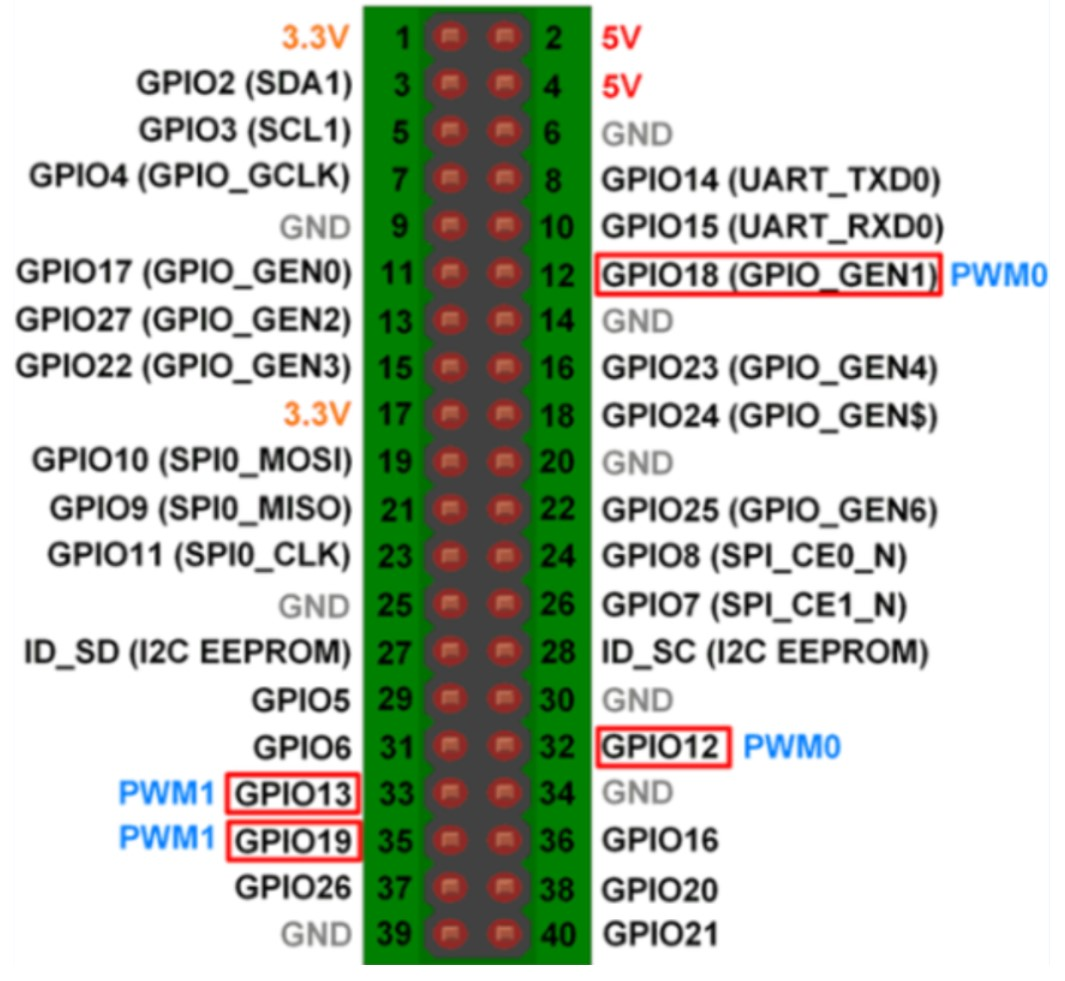
\includegraphics[width=\textwidth]{media/rp_3bp_pinout.jpg}
                \caption{Raspberry Pi 3B+ Pin-out}
                \label{fig:rp_3bp_pinout}
            \end{figure}

            The 5V, 3.3V, and Ground (0V) pins are NOT configurable. The remaining pins are general purpose pins that output 3.3V and tolerate 3.3V inputs.

            Alternative functions:
            \begin{itemize}
                \item PWM: Pulse-Width Modulation 
                \begin{itemize}
                    \item Hardware Interrupt (available on specific pins)
                    \item Software Interrupt (available on all pins)
                \end{itemize}
                \item ...
            \end{itemize}

        \subsection{Initial Configuration: Prereq. Terminology}
            \subsubsection{What is an OS?}
            \subsubsection{What is the internet?}
                Computers that are connected to each other by wire/less connection & share data form a network. 
                The internet is a large network in which your computer behaves as a \textbf{Host} or \textbf{End System}. It is connected to the internet and is a part of it.
                Deeper devices that forward data among each other and end systems are called \textbf{packet switches}. Those can be routers or link-layer switches.
                All of these components are connected via \textbf{communication links}. \\

                The internet connection is provided via national/local \textbf{ISP}s (internet service providers). ISPs are connected to one another, so the \textbf{internet} is a network of networks, and an infrastructure that is heavily relied on to provide services to applications. \\

                \textbf{Distributed applications} involve multiple end systems that exchange data. For example, YouTube, any social media application, Amazon music, and etc. rely on the internet to provide them an interface to send and receive data.

            \subsubsection{What is an IP address?}
                An (IP) Internet Protocol Address is a digital address that identifies your device’s location.
                A \textbf{protocol} is set of rules and messages that form the internet standard. 
                Your device directly requests your Internet Service Provider (ISP), which grants it access to the web. \\

                There is a vast number of available IP addresses, and reserving some addresses or ranges (called blocks) can simplify management of DHCP (Dynamic Host Configuration Protocol) Servers, prevent programming conflicts and improve network security and efficiency. 

            \subsubsection{Loopback IP Addresses}
                Among the reserved IP’s, 127.0.01 is a reserved loopback address. 
                A loopback IP address always refer to the local computer (here, local refers to the computer (the raspberry pi) that contains the hosts file), a.k.a, data packets are always returned the computer instead of being send to the local network or the internet. Allowing the local machine to refer to itself instead of an IP address is handy when needed an interface that don’t shut down (as long as the device is up, and unless it’s set to shutdown). It’s usually used for management on routers, testing and troubleshooting network applications, and improving their performance.  \\

                Note: 127.0.0.1 ≠ localhost. Localhost refers to an entire range of IP addresses used for loopback, and 127.0.0.1 is not always usable for loopback. \\

                \noindent Ergo, do NOT change or remove the line ‘127.0.0.1 localhost’ in the hosts file.

            \subsubsection{Static IPs}
                (handy for headless setup, but prone to security issues and other troubles. also less flexible)

            \subsubsection{Architecture: Peer-to-Peer vs. Server-Client}
            \subsubsection{What is SSH?}
                The Secure Shell Protocol is a Communication Protocol (like http, https, ftp, etc) that allows access to a remote computer while encrypting your traffic. Similar services (such as telnet) are not as secure because they’re not encrypted. This included file editing, installation/running programs, deploying applications, setting up web servers, etc. It’s mostly done via a remote command line terminal, but can also be used with SCP (Secure File Copy) & GUI (Graphical User Interface) programs that allows you to drag and drop files (such as WinSCP for Windows, or FileZilla (an FTP client)). \\

                \underline{\textbf{Server Requirements:}}
                Not any machine can be logged into. The server must have sshd installed and running. SSHD (Open SSH Daemon, which listens for SSH connections) is the server, and SSH is the client.\\
                \textbf{Daemons} are programs that continuously run as background processes and wake up to handle periodic service requests. They behave as servers in a client server model.\\

                Ubuntu operating systems automatically have sshd installed. 

                The server contains a sshd config file that can be edited. One use case is editing it to disable passwords (to prevent brute-force attacks).\\

                \underline{\textbf{Client Requirements:}}
                Additionally, to access a remote server from a private laptop, a software is needed to run SSH.
                On MacOS and Linux, you can enter \texttt{ssh} in the terminal.\\
                On windows, a Linux subsystem for Windows can be installed from the Microsoft Store. However, using an application like PuTTy is more convenient.\\
                PuTTy can be installed from \ur{http://putty.org}. Beware of fake putty programs, which rather that connecting to the server, share your private key with a 3rd party who can then access your server as you.\\

                There are multiple authentication methods for logging in with SSH: 
                \begin{itemize}
                \item \textbf{Password (default):}\\
                    This method is prone to brute-force attacks or password leaks.\\
                    
                    A user exists on the remote server, and a password for that user.\\
                    Login with: \texttt{ssh <username>@<local\_ip\_address\_of\_server>} \\
                    Then enter password after prompt.\\ 
                
                \item \textbf{SSH Keys (Public / Private Key pair):}\\
                Same login as with password but bypass the password. This is done by generating a set of public & private keys on your machine.\\

                    Two files are stored on your device. One contains the private key (do NOT share), and the other has the public key. The public key can be calculated from the private key, but not vice versa, so it doesn't matter if the public key is shared.\\

                    When initiating a connection, the SSH client on your local machine reads the private key, then requests the server to connect.\\ 
                    The client provides that public equivalent of the private key. \\
                    Once the server receives the public key and accepts, it generate a random stream of characters and numbers, then uses an algorithm that encrypts that string using the public key, and can only be decrypted with the private one. \\  

                    The server sends the encrypted stream to the client, which preforms a calculation on the string and returns a result to the server. This result isn't exactly the same as the original, but can prove the client has the private key. \\

                    If the server authenticates the result, the client is allowed access.      
                    
                
                \item \textbf{Host-based:} \\
                    It goes by the host. The machine contains a file called hosts that stores any hosts that are allowed to connect to it.\\
                \end{itemize}                

                Connecting to a Raspberry Pi via SSH does not follow a peer-to-peer (P2P) architecture. In a p2p network, each peer is equal to the others, with no admin. Each computer behaves as a client and a server.
                
                Connecting to the Raspberry Pi via SSH is a Client-Server model. When you enter the ssh command on your PC’s terminal, it plays the role of a client (or “host”). It sends a request to the server (the RP) which accepts the connection and allows the client access.

        \subsubsection{TCP/IP Protocol Suite}
            \textbf{Note:}\\
            This section is not a pre-requisite for setting up the raspberry pi, but may come in handy for understanding ROS. Feel free to skip this section for now and return later.\\ 
        
            TCP/IP is a network model designed to support network communication, even for computers with different manufacturers.\\ 

            \begin{figure}[htbp]
            \centering
            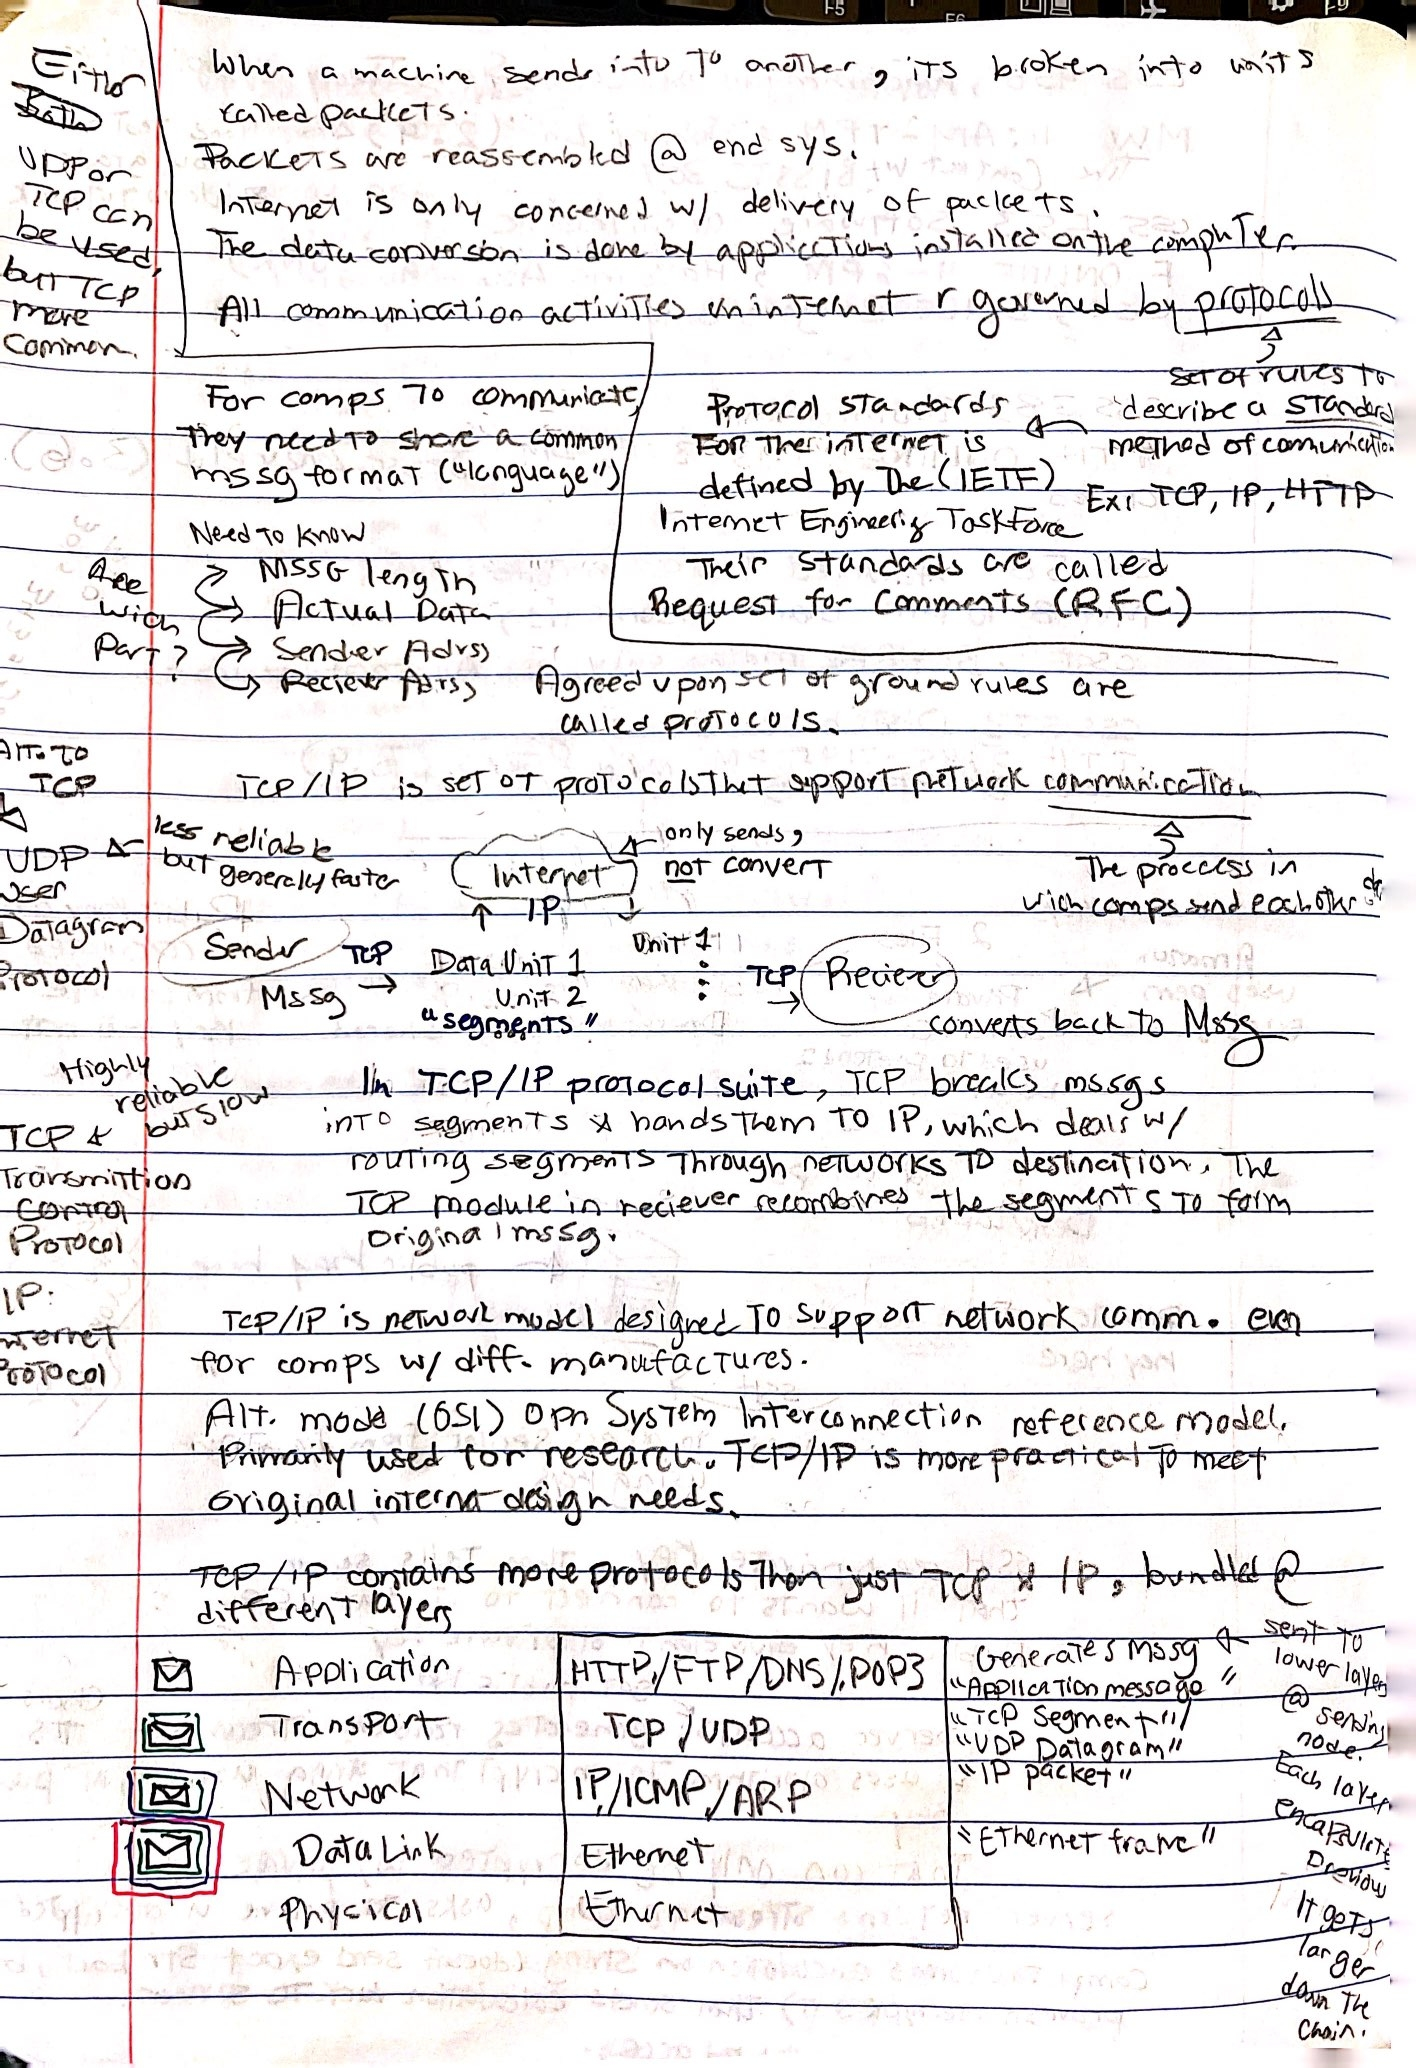
\includegraphics[width=1.2\textwidth]{media/temp_tcpip_notes.jpg}
            \label{fig:TCP/IP Notes placeholder}
            \caption{Coming soon}
            \end{figure}

        
    \subsection{Initial Configuration: Burning an OS, Images, and Related}  
        \subsubsection{Reasoning behind using the Ubuntu Server 20.04 LTS (64-bit) OS}
            Further explanation will be given later on what ROS is and the decision behind using ROS2. For now, know that ROS (Robot Operating System) is a popular middleware (not an actual OS) as it tremendously supports development with its libraries and tools, and is free.
            Not all distributions of ROS2 are compatible with the raspberry pi. According to the current documentation ROS 2 on Raspberry Pi, ROS2 is supported on 32 and 64 bit ARM processors (with 64-bit receiving more support). According to the rpi3 b+ product brief, the raspberry pi 3 B+ contains a 64-bit ARM-based processor.
            All ROS distributions are supported by a version Ubuntu LTS, and foxy needs Ubuntu 2.04 LTS (long-term support). Because the raspberry pi will be boarded, the desktop version is unnecessary as it contains unneeded packages. 

        \subsection{Reformatting the SD into FAT32}
            \subsubsection{What is a partition?}
                A \textbf{partition} is a logical division of a hard disk drive. Usually when working with a "drive", you're actually working with a partition that's assigned a drive letter (for ex, W:/). Not all partitions are assigned a drive letter, such as a recovery partition if created.\\

                Partitions are necessary for operating an OS, which needs a place to store it's file, including it's root directory.\\

                4 \underline{primary partitions} can...
                
            \subsubsection{What is a file system?}
            \subsubsection{Why FAT32?}
            \subsubsection{Formatting the SD}
            \subsubsection{Common Problems}
                \begin{itemize}
                    \item Fixing read-only (physical/not)
                    \item Recovering data from formatted SD
                \end{itemize}
        
        \subsection{Burning images onto the SD card}
            There are two popular imagers for flashing the SD card, balenaEtcher - a fast and reliable imager, and the raspberry pi imager, which makes it easy to set up the hostname, user, password, WiFi and ssh before boot. \\

        \underline{\textbf{Method A: Raspberry Pi Imager}}\\
        Install the raspberry pi imager: \url{https://www.raspberrypi.com/software/}\\
        
        On the raspberry pi imager, select\\
        Operating System $\rightarrow$ Other general-purpose OS  $\rightarrow$ Ubuntu $\rightarrow$ Ubuntu Server 20.04 LTS (64-bit) 
        
       \begin{figure}[h]
            \centering
            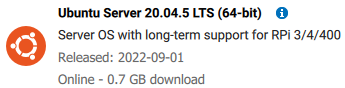
\includegraphics[width=0.7\textwidth]{media/ubuntu_rp_imager.png}
            \label{fig:rp-ubuntu-server}
        \end{figure}
    
        Check that it is compatible with your model. \\
        Enter Ctrl+Shift+X to open settings. \\
        Set (and note your) hostname, username, and password and locale settings. \\
        Enable SSH (use password authentication). \\
        
        Once done, eject the SD card and remove. \\ 
    
    
        \underline{\textbf{Method B: balenaEtcher}} \\
        Install the balenaEtcher imager: \url{https://www.balena.io/etcher} \\
    
        Download Ubuntu Server 22.04 LTS, 64-bit: \\ \url{https://ubuntu.com/download/raspberry-pi} \\
        (check compatibilities) and flash onto the SD card with the imager. \\
    
        \begin{figure}[h]
            \centering
            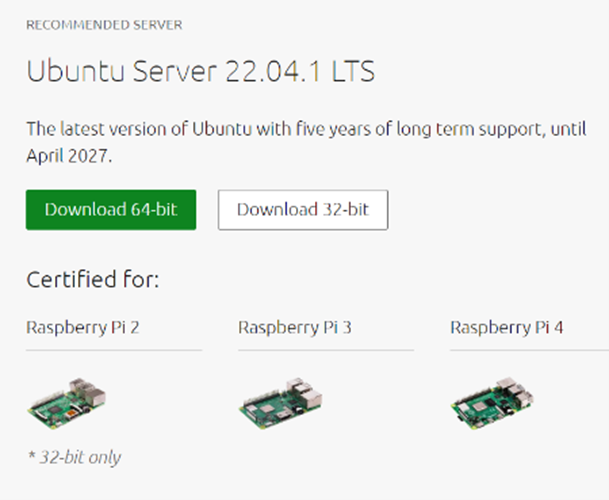
\includegraphics[width=0.7\textwidth]{media/ubuntu_server_image.png}
            \label{fig:ubuntu-server}
        \end{figure}
    
        
        Using an SD adapter, mount SD onto laptop.\\
        Flash from file: Select ubuntu-20.04.5-preinstalled-server-arm64+raspi.img.xz \\
        Select target: SDHC Card \\
        
        Check the drive letter is correct!
        If it was hidden, it’s very unlikely to be your SD. \\
        
        Do not eject the SD card yet, since SSH configurations must be done \underline{before} the first boot.
        Follow additional instructions to set up user after starting up the display. \\
        

    \subsection{\textbf{Optional:} Connecting a Display to the RP}
            \subsubsection{\textbf{Method 1: HDMI}}

            \textbf{Do not power the RP yet.} \\
                
            \subsubsection{\textbf{Method 2: Official RP Touchscreen Display}}                   
            \url{https://thepihut.com/products/official-raspberry-pi-7-touchscreen-display}\\

            \begin{figure}[htbp]
            \centering
            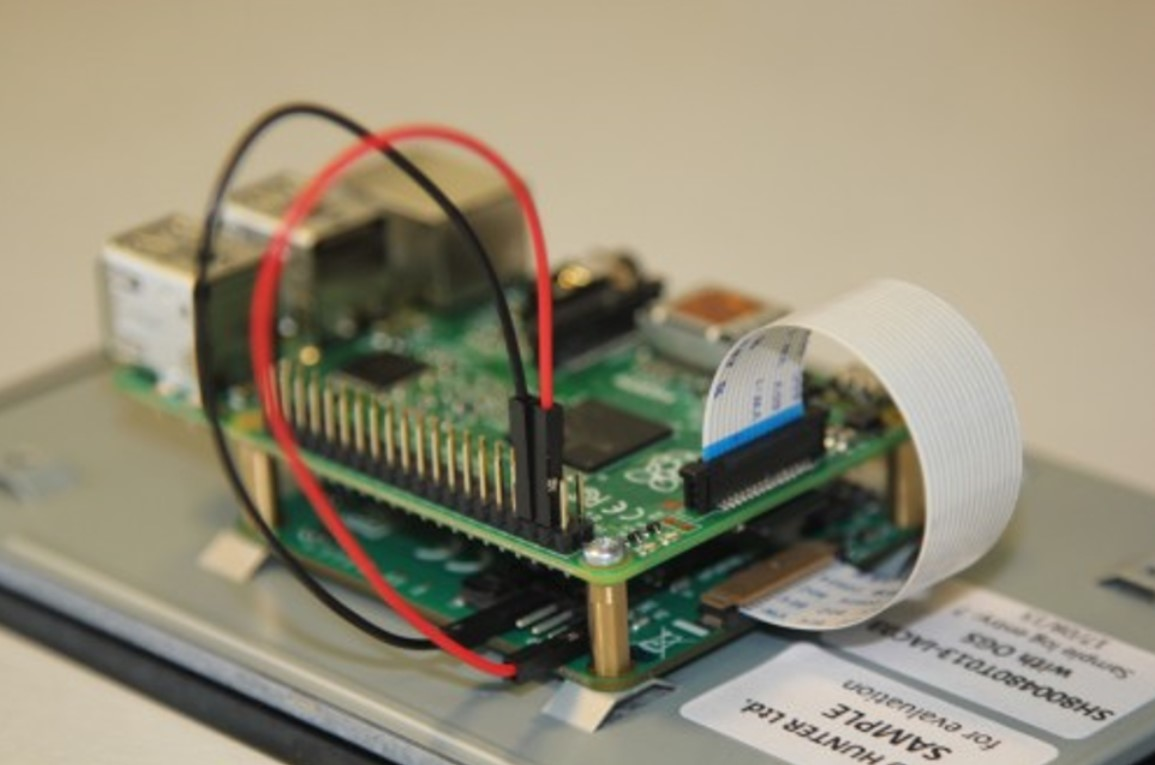
\includegraphics[width=\textwidth]{media/rp_display_wiring.jpg}
            \caption{Wiring the Raspberry Pi Display}
            \label{fig:rp_display_wiring}
            \end{figure}

            \noindent Although different raspberry pi models have generally different pinouts for GPIO, they share the same pins for power and ground. 
            Attach the jumper cables as seen in the image to provide power for the display. \\

            \noindent The display’s ribbon cable (transmitter) must be attached to the correct connector on the raspberry pi – one is for the display and the other for a camera. Their labels can be seen on the board. \\

            \noindent Alternatively, an HDMI cable can be used to connect to a monitor.
            To connect to keyboard, insert it’s USB cable or dongle into USB ports.
            Before powering the device, mount the SD onto raspberry pi. \\
                
            \noindent \textbf{Do not power the RP yet.} 

        \subsection{Missing Display or Keyboard: Headless Setup} 
        

        \subsection{User Configurations}
        \underline{Common Mistakes}:
        \begin{itemize}
            \item Ubuntu login is asking for the username, not the password.
            \item When asked to set a new password, you are first asked to enter the current password. Enter "ubuntu", then type in the new password.
        \end{itemize}
        
        \textbf{Create a new admin user:}\\
        \texttt{sudo adduser <username>} \\

        \noindent Sample: \\
        \texttt{ sudo adduser piparty} \
        \begin{flushleft}
            \begin{tabular}{|c|c|}
                \hline
                Username & piparty \\
                \hline
                Password & ****** \\
                \hline
                Full Name & UWB HackRover RP 2 \\
                \hline
                Room \# & DISC 270 \\
                \hline
            \end{tabular}
        \end{flushleft} 


        \noindent \textbf{Add new user to sudo group} (Sample)\\
        \texttt{sudo usermod -aG sudo piparty} \\
        aG stands for append to group \\
        
        \noindent \textbf{Switch to new user:} \\
        \texttt{su - <username>}\\
        Sample: \texttt{su - piparty} \\
        
        \underline{\textbf{Change hostname }}(optional)\\
        \textbf{Enter root user:} \texttt{sudo su} \\
        \textbf{Edit hostname files:} \texttt{nano /etc/hostname} \\
        
        Change hostname as desired. It should:
        \begin{itemize}
            \item Not be same as other devices
            \item Not use special characters or spaces
            \item Not start with or consist only of numbers
            \item Be short, descriptive, and memorable
            \item Stick to lowercase letters (although uppercase is fine)
        \end{itemize}

        
        \noindent Sample hostname: hrrp2 (for:  HackRover raspberry pi 2)\\
         
        \noindent\textbf{Save:} Ctrl+S \\
        \textbf{Exit:} Ctrl+X \\
        
        \begin{mdframed}
            \underline{\textbf{Disabling default user:}}\\ 

            \begin{tabular}{ll}
                \textbf{Switch to root user:} & \texttt{sudo su}\\
                \textbf{Lock root user’s password:} & \texttt{passwd -l ubuntu}\\
            \end{tabular}\\
            
            If successful, the following message will be displayed: \\
            \texttt{passwd: password expiry information changed.}\\

           \textbf{ Exit root user:} \texttt{         exit}\\

           Until the root user is re-enabled, it will no longer be possible to ssh into the raspberry pi with just the IP Since it automatically try to log in as root (which's password you disabled).\\
           (\texttt{ssh <ip>} will no longer work).\\

           You will need to specify the user with\\ \texttt{ssh <username>@<ip-address>}\\

        \end{mdframed}\\

        \begin{mdframed}
            \underline{\textbf{Re-enabling default user:}}\\ 
            \begin{tabular}{ll}
                Switch to root user: & \texttt{sudo su}\\
                Unlock root (“ubuntu”) user’s password: & \texttt{passwd -u ubuntu}\\
                Exit root user: & \texttt{exit}\\
            \end{tabluar}\\

        \end{mdframed}\\


    


    \subsection{Configuring Network and Remotely Accessing the RP via SSH}
        It is necessary to first find which tool is managing the network interface:
        \begin{lstlisting}
            ls -alh /etc/network/interfaces.d
        \end{lstlisting}
        If there is no such file or directory, the interfaces configuration is NOT stored there. Try
        
        \begin{lstlisting}[language=bash]
            ls -alh /etc/netplan
        \end{lstlisting}

    \subsection{Backing up images}
    \subsection{Debugging}
    sshing with -v, -vv, -vvv...
    
    \subsection{References/Resources}
        \textbf{Sources:}
        \begin{itemize}
          \item ARM vs x86: 
          \url{https://www.redhat.com/en/topics/linux/ARM-vs-x86}
          \item Raspberry Pi 3 Model B+ Specs: \url{https://datasheets.raspberrypi.com/rpi3/raspberry-pi-3-b-plus-product-brief.pdf}
          \item Raspberry Pi Comparison Chart: \url{https://cdn.shopify.com/s/files/1/0176/3274/files/Raspberry-Pi-Comparison_r4.pdf?3484}
          \item RP Documentation: \url{https://www.raspberrypi.com/documentation/computers/raspberry-pi.html}
          \item RP 3B+ Product Brief:
          \url{https://datasheets.raspberrypi.com/rpi3/raspberry-pi-3-b-plus-product-brief.pdf}
          \item ROS2 Distributions: \url{http://wiki.ros.org/Distributions}
          \item ROS2 on RP: \url{https://docs.ros.org/en/foxy/How-To-Guides/Installing-on-Raspberry-Pi.html}
          \item (Raspberry pi display) \url{https://www.raspberrypi.com/documentation/accessories/display.html}
        \item (Create new RP user) \url{https://raspberrytips.com/new-user-on-raspberry-pi/}
        \item \url{https://askubuntu.com/questions/754213/what-is-difference-between-localhost-address-127-0-0-1-and-127-0-1-1}
        \item (Debian Reference Manual – Network Configuration) \url{https://qref.sourceforge.net/quick/ch-gateway.en.html}
        \item (IP Address function, types, protection) \url{https://www.codecademy.com/resources/blog/ip-address/}
        \item \url{https://www.geeksforgeeks.org/what-is-an-ip-address/}
        \item \url{https://www.howtogeek.com/789017/what-is-the-127.0.0.1-ip-address-and-how-do-you-use-it/}
        \item \url{https://www.howtogeek.com/784196/how-to-edit-the-hosts-file-on-windows-10-or-11/}
        \item \url{https://learningnetwork.cisco.com/s/question/0D53i00000Kt6ZUCAZ/what-is-loopback-addresseswhat-is-the-purpose-of-using-it-and-when-can-we-use-it}
        \item (127.0.0.1 vs localhost) \url{https://phoenixnap.com/kb/localhost-vs-127-0-0-/}
        \item (IPv4 vs IPv6) \url{https://phoenixnap.com/blog/ipv4-vs-ipv6}
        \item Linux SSH manual page & options \url{https://man7.org/linux/man-pages/man1/ssh.1.html}
        \item (SSH Keys) \url{https://www.youtube.com/watch?v=dPAw4opzN9g}
        \item (SSH Crash Course) \url{https://www.youtube.com/watch?v=hQWRp-FdTpc}
        \item (SSH tunneling) \url{https://www.ssh.com/academy/ssh/tunneling}
        \item (Reverse SSH tunneling) \url{https://www.howtogeek.com/428413/what-is-reverse-ssh-tunneling-and-how-to-use-it/}
        \item (VPN vs SSH tunnel) \url{https://www.howtogeek.com/118145/vpn-vs.-ssh-tunnel-which-is-more-secure/}
        \item (Daemon) \url{https://www.techtarget.com/whatis/definition/daemon}
        \item (Client-Server Model) \url{https://www.techtarget.com/searchnetworking/definition/client-server}
        \item (Network Protocols Fundamentals) \url{https://www.youtube.com/watch?v=E5bSumTAHZE}
        \item (TCP IP) \url{https://www.youtube.com/watch?v=2QGgEk20RXM}
        \item (TCP, IP, UDP) \url{https://www.vskills.in/certification/tutorial/tcp-ip-packet-formats-and-ports/}
        \item (TCP/IP function, layers vs OSI model) \url{https://www.techtarget.com/searchnetworking/definition/TCP-IP}
        \item (DNS) \url{https://www.howtogeek.com/122845/htg-explains-what-is-dns/}
        \item \url{https://www.digitalcitizen.life/}
        \item \url{https://www.lifewire.com/what-is-a-partition-2625958}
        \item \url{https://www.easeus.com/diskmanager/file-system.html}
        \item \url{https://www.lifewire.com/virtual-machine-4147598}
        \item \url{https://www.lifewire.com/what-is-a-root-folder-or-root-directory-2625989}
        \item \url{https://raspberrypi.stackexchange.com/questions/44074/raspberry-pi-3-why-the-fat-partition}
        \item \url{https://www.tomshardware.com/reviews/local-area-network-wi-fi-wireless,3020-2.html}
        \item \url{https://www.cloudflare.com/learning/ddos/glossary/tcp-ip/}
        \item \url{https://www.cloudflare.com/learning/network-layer/what-is-a-lan/}
        \item \url{https://www.networkstraining.com/peer-to-peer-vs-client-server-network/}
        \item \url{https://youtu.be/0Sffl7YO0aY}
        \item \url{https://www.geeksforgeeks.org/tcp-server-client-implementation-in-c/}
        \item \url{https://www.hostinger.com/tutorials/what-is-ubuntu}
        \item (Headless Ubuntu Setup) \url{https://www.youtube.com/watch?v=ZE2HmyI0t7U}
        \item \url{https://netplan.io/examples}
        \end{itemize}



 %============================================================
 \pagebreak

\section{``ROS2''}
\subsection*{Summary}
	\subsection{``Popular open-source robotics frameworks''}
	ROS and YARP...

        \subsection{``What is ROS?''}
        Although ROS stands for Robot Operating System, it’s not an OS  like Ubuntu or Raspbian. According to its documentation, ROS is an open-source meta-operating system that’s build on top of the operating system.\\
        \textbf{Open source} just means the source code is freely accessible for use and modification.\\
        A \textbf{meta operating system} is... \\
        
        Although it’s not described as such in the documentation (and thus shouldn’t be called so for clarity), some users may refer to is as a framework or a middleware system, since it shares some of their characteristics.\\ 
        \textbf{Middleware} is software that enables communication and management of data in distributes applications. A \textbf{distributed application} is software that runs on multiple machines (physical or virtual) within a network. 


        \subsection{``Installing ROS2 Foxy (via Debian packages)''}
        It is recommended to install foxy via Debian packages since it automatically installs necessary dependencies, and updates when the system does. Instructions can be found in the documentation here: \\ \url{https://docs.ros.org/en/foxy/Installation/Ubuntu-Install-Debians.html}. \\

        If, for some reason, it is not possible to install via Debian packages, alternative instructions are provided in the documentation: \\ \url{https://docs.ros.org/en/foxy/Installation.html}.\\ 
        
        The following is specified for a Debian-based installation. \\
		\subsubsection{ROS2 on the raspberry pi}

		\subsubsection{ROS2 on VirtualBox (PC)}

            \subsection{Installation Issues}
            \begin{itemize}
                \item \textbf{E: Unable to locate package ros-foxy-ros-base}\\
                Check your version of Ubuntu: 
                \begin{verbatim}
                    lsb_release -a
                \end{verbatim}\\


                It should be \underline{version 22.04 LTS}, with \underline{codename focal}. If that's not the case, the SD card will need to be re-burned with the correct image.

                \item \textbf{ModuleNotFoundError: No module named 'RPi'}\\
                Install with\\
                \begin{verbatim}
                    sudo apt-get update
                    sudo apt-get install python3-rpi.gpio
                \end{verbatim}\\

            \end{itemize}

    \subsection{References/Resources}
        \begin{itemize}
            \item \url{42-	https://www.redhat.com/en/topics/open-source/what-is-open-source}
            \item \url{43-	https://answers.ros.org/question/12230/what-is-ros-exactly-middleware-framework-operating-system/ }
        \end{itemize}
	
 %============================================================
\pagebreak

\section{``Interfacing the BTS796043A with the RP''}
    \subsection*{Summary}

    \subsection*{Note}
    Refer to the data sheet here: \\ \url{http://www.robotpower.com/downloads/BTS7960_v1.1_2004-12-07.pdf}

    \subsubsection{What is a motor driver?}
        A motor driver converts low current to high current signals for motors. They're used because micro controllers are needed to send a signal to the motor  but cannot provide enough voltage. 

    \subsection{The Wiring and The Code}
    \subsubsection{Whyring: Specifications of the BTS796043A and the RP}

    \begin{figure}[!htb]
    \centering
    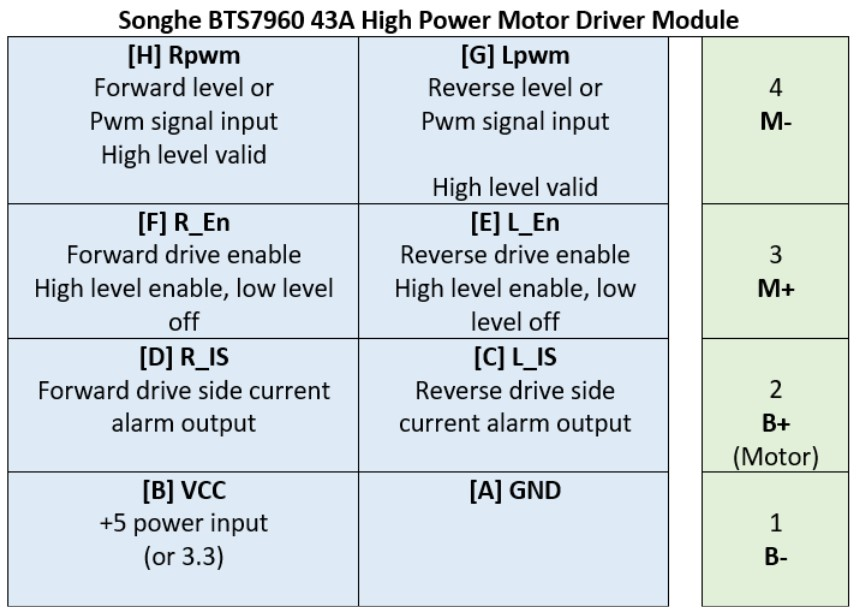
\includegraphics[width=\linewidth]{media/bts7960_pins.jpg}
    \caption{BTS7960 motor driver pins.}
    \label{fig:bts7960_pins}
    \end{figure}
    \newline
    
    Recall that the GPIO pins of raspberry pi output 3.3V. Because of this detail, the BTS's VCC needs to receive power from the 3.3V pin, not the 5V for it to work.

        \begin{table}[h]
        \centering
        \begin{tabular}{|l|l|}
        \hline
        \textbf{BTS7960} & \textbf{Power Supply} \\
        \hline
        Motor+ & Power Supply \\
        \hline
        Motor- & Power Supply \\
        \hline
        \end{tabular}
        \label{tab:motor}
        \end{table}
        
        \begin{table}[h]
        \centering
        \begin{minipage}{.35\linewidth}
        \centering
        \begin{tabular}{|l|l|}
        \hline
        \textbf{BTS} & \textbf{RP} \\
        \hline
        Rpwm & GPIO18 [12] \\
        \hline
        R\_En & GPIO20 [38] \\
        \hline
        R\_IS & GPIO6 [31] \\
        \hline
        VCC & 3.3V [1] \\
        \hline
        \end{tabular}
        \label{tab:right}
        \end{minipage}
        \begin{minipage}{.3\linewidth}
        \centering
        \begin{tabular}{|l|l|}
        \hline
        \textbf{BTS} & \textbf{RP} \\
        \hline
        Lpwm & GPIO12 [32] \\
        \hline
        L\_En & GPIO21 [40] \\
        \hline
        L\_IS & GPIO5 [29] \\
        \hline
        GND & GND [6] \\
        \hline
        \end{tabular}
        \label{tab:left}
        \end{minipage}
        \caption{Wiring Sample}
        \label{tab:pwm}
        \end{table}

        \subsubsection{Practices}
        (Use GPIO.BCM, not .BOARD)
        
        \subsubsection{HIGH and LOW vs Changing Speeds}
        \underline{\textbf{High/Low}}\\
            (Code snippet incoming...)\\
            
            Cannot embed videos yet, see: \url{https://www.overleaf.com/learn/latex/Questions/How_can_I_embed_a_video_in_my_PDF_using_LaTeX%3F}.\\

            For now, please refer to the file \url{rp_motor_high_low.MOV} in the media folder.\\

        \underline{\textbf{Using PWM}}\\
            (Work in process) \\
            
    \subsection{Code to a Node}
         
    \subsection{References/Resources}
    \begin{itemize}
        \item Motor Controllers vs Motor Drivers: \url{https://core-electronics.com.au/guides/motor-drivers-vs-motor-controllers/}
        \item PWM: \url{https://forums.raspberrypi.com/viewtopic.php?t=197498}
        \item Amazon Songhe BTS7960 43A High Power Motor Driver Module: \\
        \url{https://www.amazon.com/BTS7960-Driver-Module-Arduino-Current/dp/B07TFB22H5/}
        \item Non-PWM Control and Reason for VCC to 3.3V Pin: \\ \url{https://electronics.stackexchange.com/questions/398556/how-to-control-a-motor-driver-bts7960-without-pwm}
        \item 32 RPM HD Premium Planetary Gear Motor w/Encoder: \url{https://www.servocity.com/32-rpm-hd-premium-planetary-gear-motor-w-encoder/}
        \item NE12 Magnetic Encoder Use Parameter: \\ \url{https://www.servocity.com/content/downloads/ne12_-_use_parameter.pdf}

    \end{itemize}
 %============================================================
\end{document}
